\exercisesheader{}

% 3

\eoce{\qt{Air pollution and birth outcomes, study components\label{study_components_airpoll}} 
Researchers collected data to examine the relationship between air pollutants 
and preterm births in Southern California. During the study air pollution levels 
were measured by air quality monitoring stations. Specifically, levels of carbon 
monoxide were recorded in parts per million, nitrogen dioxide and ozone in parts 
per hundred million, and coarse particulate matter (PM$_{10}$) in $\mu g/m^3$. 
Length of gestation data were collected on 143,196 births between the years 1989 
and 1993, and air pollution exposure during gestation was calculated for each 
birth. The analysis suggested that increased ambient PM$_{10}$ and, to a lesser 
degree, CO concentrations may be associated with the occurrence of preterm births.\footfullcite{Ritz+Yu+Chapa+Fruin:2000}
\begin{parts}
\item Identify the main research question of the study.
\item Who are the subjects in this study, and how many are included?
\item What are the variables in the study? Identify each variable as numerical or 
categorical. If numerical, state whether the variable is discrete or continuous.
If categorical, state whether the variable is ordinal.
\end{parts}
}{}

% 4

\eoce{\qt{Buteyko method, study components\label{study_components_buteyko}} 
The Buteyko method is a shallow breathing technique developed by Konstantin 
Buteyko, a Russian doctor, in 1952. Anecdotal evidence suggests that the Buteyko 
method can reduce asthma symptoms and improve quality of life. In a scientific 
study to determine the effectiveness of this method, researchers recruited 600 
asthma patients aged 18-69 who relied on medication for asthma treatment. These 
patients were randomnly split into two research groups: one practiced the Buteyko 
method and the other did not. Patients were scored on quality of life, activity, 
asthma symptoms, and medication reduction on a scale from 0 to 10. On average, 
the participants in the Buteyko group experienced a significant reduction in 
asthma symptoms and an improvement in quality of life.\footfullcite{McDowan:2003} 
\begin{parts}
\item Identify the main research question of the study.
\item Who are the subjects in this study, and how many are included?
\item What are the variables in the study? Identify each variable as numerical or 
categorical. If numerical, state whether the variable is discrete or continuous.
If categorical, state whether the variable is ordinal.
\end{parts}
}{}

% 5

\eoce{\qt{Cheaters, study components\label{study_components_cheaters}} 
Researchers studying the relationship between honesty, age and self-control 
conducted an experiment on 160 children between the ages of 5 and 15. 
Participants reported their age, sex, and whether they were an only child 
or not. The researchers asked each child to toss a fair coin in private and 
to record the outcome (white or black) on a paper sheet, and said they 
would only reward children who report white.\footfullcite{Bucciol:2011} 
\begin{parts}
\item Identify the main research question of the study.
\item Who are the subjects in this study, and how many are included?
\item The study's findings can be summarized as follows: "Half the students were 
explicitly told not to cheat and the others were not given any explicit 
instructions. In the no instruction group probability of cheating was found to 
be uniform across groups based on child's characteristics. In the group that was 
explicitly told to not cheat, girls were less likely to cheat, and while rate 
of cheating didn't vary by age for boys, it decreased with age for girls." 
How many variables were recorded for each subject in the study in order to 
conclude these findings? State the variables and their types.
\end{parts}
}{}

\D{\newpage}

% 6

\eoce{\qt{Stealers, study components\label{study_components_stealers}} 
In a study of the relationship between socio-economic class and unethical 
behavior, 129 University of California undergraduates at Berkeley were asked 
to identify themselves as having low or high social-class by comparing 
themselves to others with the most (least) money, most (least) education, and 
most (least) respected jobs. They were also presented with a jar of 
individually wrapped candies and informed that the candies were for children
in a nearby laboratory, but that they could take some if they wanted. After 
completing some unrelated tasks, participants reported the number of candies 
they had taken.\footfullcite{Piff:2012} 
\begin{parts}
\item Identify the main research question of the study.
\item Who are the subjects in this study, and how many are included?
\item The study found that students who were identified as upper-class took more 
candy than others. How many variables were recorded for each subject in the study 
in order to conclude these findings? State the variables and their types.
\end{parts}
}{}

% 7

\eoce{\qt{Migraine and acupuncture,
    Part II\label{migraine_and_acupuncture_exp_resp}}
Exercise~\ref{migraine_and_acupuncture_intro}
introduced a study exploring whether acupuncture had any
effect on migraines.
Researchers conducted a randomized controlled study
where patients were randomly assigned to one of two groups:
treatment or control.
The patients in the treatment group received acupuncture
that was specifically designed to treat migraines.
The patients in the control group received placebo acupuncture
(needle insertion at non-acupoint locations).
24 hours after patients received acupuncture, they were asked 
if they were pain free.
What are the explanatory and response variables in this study?
}{}

% 8

\eoce{\qt{Sinusitis and antibiotics,
    Part II\label{sinusitis_and_antibiotics_exp_resp}} 
Exercise~\ref{sinusitis_and_antibiotics_intro}
introduced a study exploring the effect of antibiotic treatment
for acute sinusitis.
Study participants either received either a 10-day course of
an antibiotic (treatment)
or a placebo similar in appearance and taste (control).
At the end of the 10-day period, patients were asked if
they experienced improvement in symptoms.
What are the explanatory and response variables in this study?
}{}

% 9

\eoce{\qt{Fisher's irises\label{fisher_irises}} Sir Ronald Aylmer Fisher was an 
English statistician, evolutionary biologist, and geneticist who worked on a 
data set that contained sepal length and width, and petal length and width from 
three species of iris flowers (\textit{setosa}, \textit{versicolor} and 
\textit{virginica}). There were 50 flowers from each species in the data set. 
\footfullcite{Fisher:1936} \\
\noindent\begin{minipage}[c]{0.48\textwidth}
\begin{parts}
\item How many cases were included in the data?
\item How many numerical variables are included in the data? Indicate what 
they are, and if they are continuous or discrete.
\item How many categorical variables are included in the data, and what are 
they? List the corresponding levels (categories).
\end{parts}
\end{minipage}
\begin{minipage}[c]{0.01\textwidth}
\ 
\end{minipage}
\begin{minipage}[c]{0.2\textwidth}
\begin{center}
\includegraphics[width = \textwidth]{ch_intro_to_data/figures/eoce/fisher_irises/irisversicolor.jpg}
\end{center}
\end{minipage}
\begin{minipage}[c]{0.01\textwidth}
\ 
\end{minipage}
\begin{minipage}[c]{0.23\textwidth}
{\raggedright\footnotesize Photo by Ryan Claussen 
(\oiRedirect{textbook-flickr_ryan_claussen_iris_picture}{http://flic.kr/p/6QTcuX}) 
\oiRedirect{textbook-CC_BY_SA_2}{CC~BY-SA~2.0~license}}
\end{minipage}
}{}

% 10

\eoce{\qt{Smoking habits of UK residents\label{smoking_habits_UK_datamatrix}} A survey 
was conducted to study the smoking habits of UK residents. Below is a data 
matrix displaying a portion of the data collected in this survey. Note that 
``$\pounds$" stands for British Pounds Sterling, ``cig" stands for cigarettes, 
and ``N/A'' refers to a missing component of the data. \footfullcite{data:smoking}
\begin{center}
\scriptsize{
\begin{tabular}{rccccccc}
\hline
	& sex 	 & age 	& marital 	& grossIncome 					     & smoke & amtWeekends	& amtWeekdays \\ 
\hline
1 	& Female & 42 	& Single 	& Under $\pounds$2,600 			     & Yes 	 & 12 cig/day   & 12 cig/day \\ 
2 	& Male	 & 44	& Single 	& $\pounds$10,400 to $\pounds$15,600 & No	 & N/A 			& N/A \\ 
3 	& Male 	 & 53 	& Married   & Above $\pounds$36,400 		     & Yes 	 & 6 cig/day 	& 6 cig/day \\ 
\vdots & \vdots & \vdots & \vdots & \vdots 				             & \vdots & \vdots 	    & \vdots \\ 
1691 & Male  & 40   & Single 	& $\pounds$2,600 to $\pounds$5,200   & Yes 	 & 8 cig/day 	& 8 cig/day \\   
\hline
\end{tabular}
}
\end{center}
\begin{parts}
\item What does each row of the data matrix represent?
\item How many participants were included in the survey?
\item Indicate whether each variable in the study is numerical or categorical. If numerical, identify as 
continuous or discrete. If categorical, indicate if the variable is ordinal.
\end{parts}
}{}

\D{\newpage}

% 11

\eoce{\qt{US Airports\label{US Airports}}
The visualization below shows the
geographical distribution of airports in the contiguous United States
and Washington, DC.
This visualization was constructed based on a dataset where
each observation is an airport.\footfullcite{data:usairports}
\begin{center}
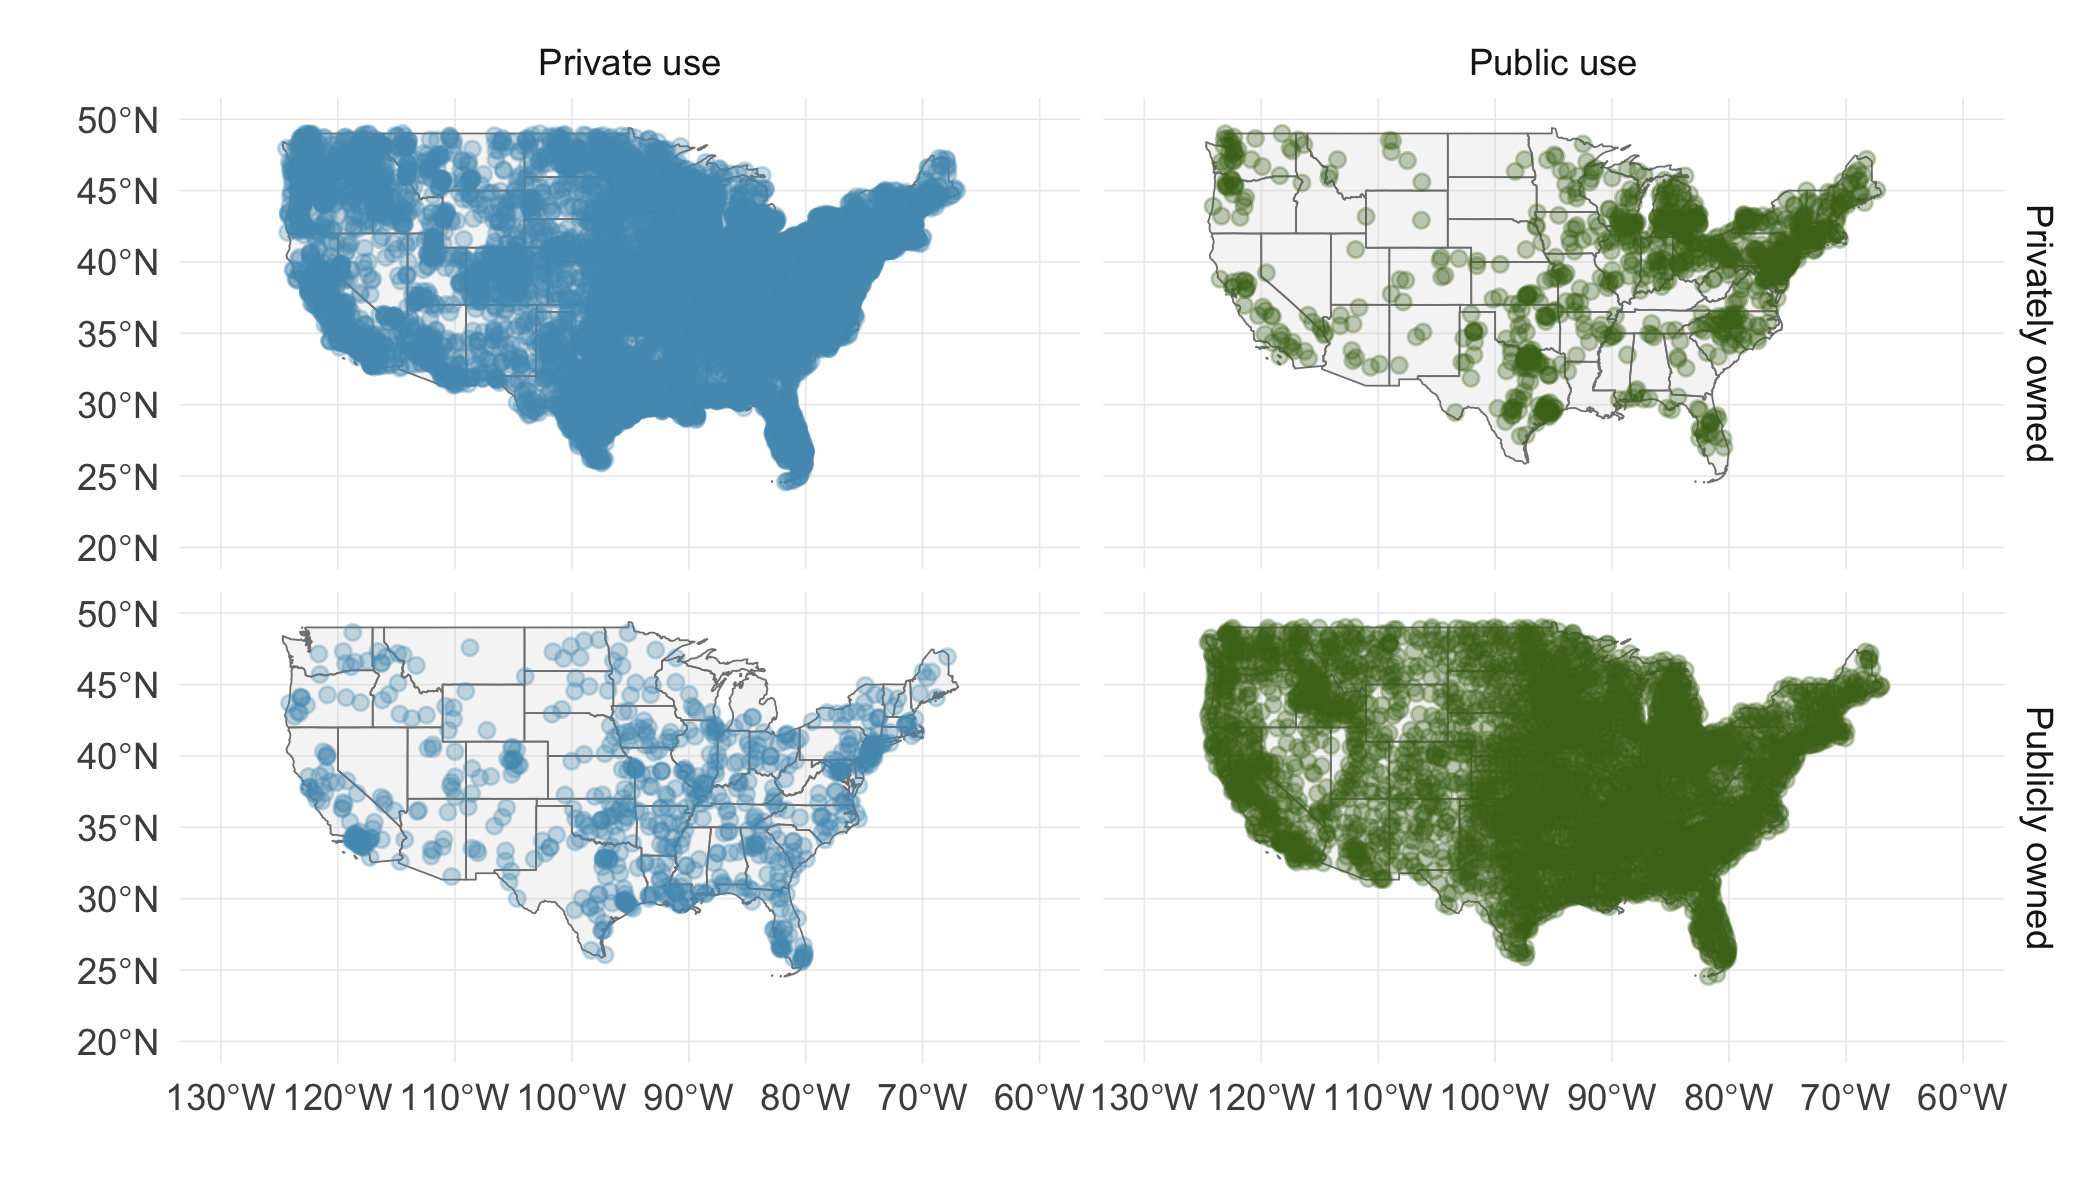
\includegraphics[width = 0.9\textwidth]{ch_intro_to_data/figures/eoce/airports/airports.png}
\end{center}
\begin{parts}
\item
    List the variables used in creating this visualization.
\item
    Indicate whether each variable in the study is numerical
    or categorical.
    If numerical, identify as continuous or discrete.
    If categorical, indicate if the variable is ordinal.
\end{parts}
}{}

% 12

\eoce{\qt{UN Votes\label{unvotes}}
The visualization below shows voting patterns in 
the United States, Canada, and Mexico in the United Nations General Assembly 
on a variety of issues. Specifically, for a given year between 1946 and 2015, 
it displays the percentage of roll calls in which the country voted yes for 
each issue. This visualization was constructed based on a dataset where each 
observation is a country/year pair.\footfullcite{data:unvotes}
\begin{center}
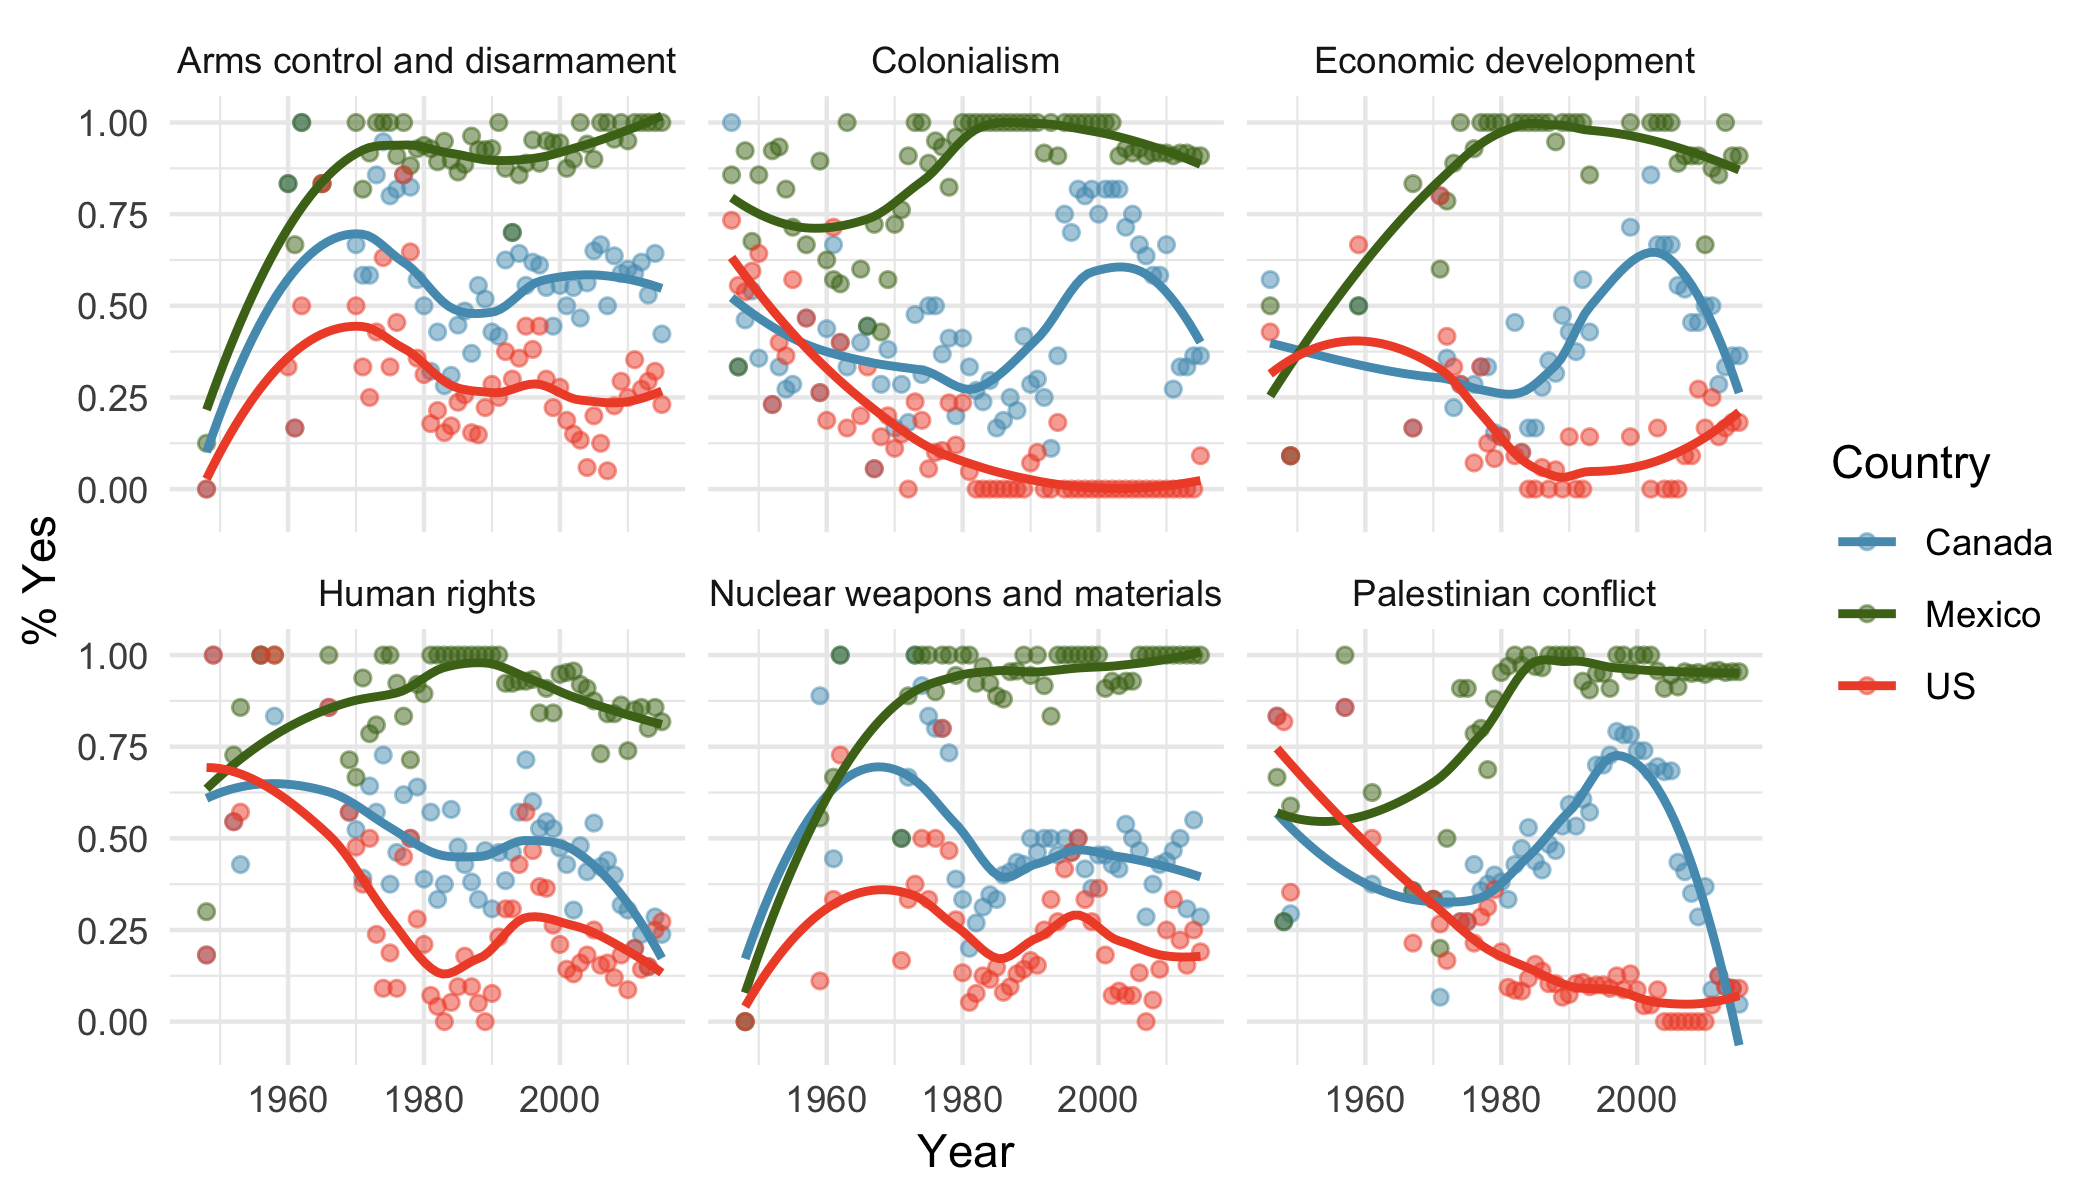
\includegraphics[width = 0.9\textwidth]{ch_intro_to_data/figures/eoce/unvotes/unvotes.png}
\end{center}
\begin{parts}
\item List the variables used in creating this visualization.
\item Indicate whether each variable in the study is numerical or categorical. 
If numerical, identify as continuous or discrete. If categorical, indicate if 
the variable is ordinal.
\end{parts}
}{}
